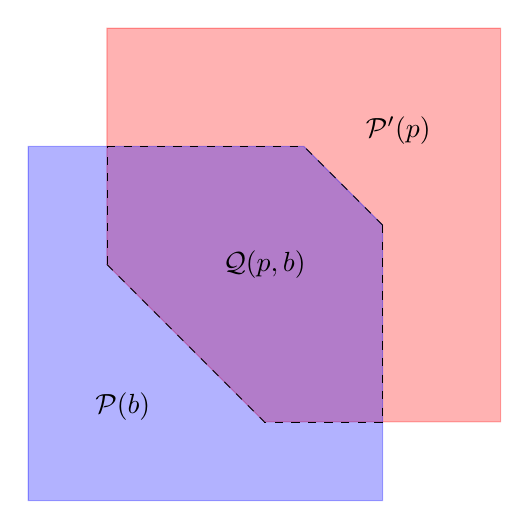
\begin{tikzpicture}

    \filldraw[opacity=0.3, red] (1,3) -- (3,1) -- (6,1) -- (6,6) -- (1,6) -- cycle;
    \filldraw[opacity=0.3, blue] (0,0) -- (4.5,0) -- (4.5,3.5) -- (3.5,4.5) -- (0,4.5) -- cycle;
    \draw[dashed, line width=0.1mm, black] (1,3) -- (3,1);
    \draw[dashed, line width=0.1mm, black] (1,3) -- (1,4.5);
    \draw[dashed, line width=0.1mm, black] (4.5,3.5) -- (3.5,4.5);
    
    \draw[dashed, line width=0.1mm, black] (1,4.5) -- (3.5,4.5);
    \draw[dashed, line width=0.1mm, black] (4.5,3.5) -- (4.5,1);
    \draw[dashed, line width=0.1mm, black] (4.5,1) -- (3,1);
    
    % \draw[-][line, width=0.1mm][black] (1,4.5) -- (1,6);
    % \draw[-][line width=0.1mm][black] (6,1) -- (3,1);
    % \draw[-][line width=0.1mm][black] (4.5,3.5) -- (4.5,0);
    % \draw[-][line width=0.1mm][black] (3.5,4.5) -- (0,4.5);
    \coordinate (A) at (1,3);
    \coordinate (B) at (3,1);
    % \filldraw (A) circle (1.5pt) node[above right] {};
    % \filldraw (B) circle (1.5pt) node[above right] {};
    \coordinate (Q) at (4.5,3.5);
    \coordinate (R) at (3.5,4.5);
    % \filldraw (Q) circle (1.5pt) node[above right] {};
    % \filldraw (R) circle (1.5pt) node[above right] {};
    \node at (1.2,1.2) {$ \mathcal{P}(b)$};
    \node at (4.7,4.7) {$ \mathcal{P}'(p)$};
    \node at (3,3) {$\mathcal{Q}(p, b)$};
\end{tikzpicture}
